% Graphic for TeX using PGF
% Title: /home/tomgli/workspace/github.com/bachopp/thesis/files/chapters/design/graphics/databaseoverview.dia
% Creator: Dia v0.97.3
% CreationDate: Sat May 14 13:53:03 2016
% For: tomgli
% \usepackage{tikz}
% The following commands are not supported in PSTricks at present
% We define them conditionally, so when they are implemented,
% this pgf file will use them.
\ifx\du\undefined
  \newlength{\du}
\fi
\setlength{\du}{15\unitlength}
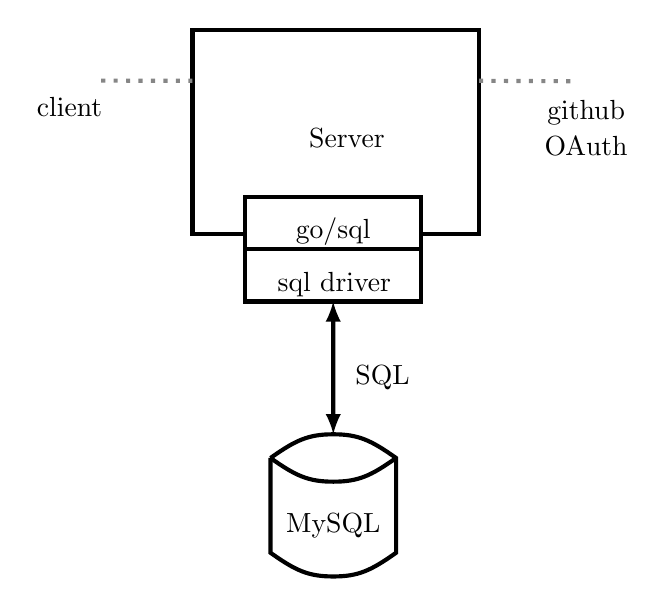
\begin{tikzpicture}
\pgftransformxscale{1.000000}
\pgftransformyscale{-1.000000}
\definecolor{dialinecolor}{rgb}{0.000000, 0.000000, 0.000000}
\pgfsetstrokecolor{dialinecolor}
\definecolor{dialinecolor}{rgb}{1.000000, 1.000000, 1.000000}
\pgfsetfillcolor{dialinecolor}
\definecolor{dialinecolor}{rgb}{1.000000, 1.000000, 1.000000}
\pgfsetfillcolor{dialinecolor}
\fill (31.545811\du,-18.175060\du)--(31.545811\du,-13.254965\du)--(38.449524\du,-13.254965\du)--(38.449524\du,-18.175060\du)--cycle;
\pgfsetlinewidth{0.100000\du}
\pgfsetdash{}{0pt}
\pgfsetdash{}{0pt}
\pgfsetmiterjoin
\definecolor{dialinecolor}{rgb}{0.000000, 0.000000, 0.000000}
\pgfsetstrokecolor{dialinecolor}
\draw (31.545811\du,-18.175060\du)--(31.545811\du,-13.254965\du)--(38.449524\du,-13.254965\du)--(38.449524\du,-18.175060\du)--cycle;
% setfont left to latex
\definecolor{dialinecolor}{rgb}{0.000000, 0.000000, 0.000000}
\pgfsetstrokecolor{dialinecolor}
\node at (34.997667\du,-15.520012\du){};
% setfont left to latex
\definecolor{dialinecolor}{rgb}{0.000000, 0.000000, 0.000000}
\pgfsetstrokecolor{dialinecolor}
\node[anchor=west] at (34.087695\du,-15.571132\du){Server};
\pgfsetlinewidth{0.100000\du}
\pgfsetdash{}{0pt}
\pgfsetdash{}{0pt}
\pgfsetbuttcap
\pgfsetmiterjoin
\pgfsetlinewidth{0.100000\du}
\pgfsetbuttcap
\pgfsetmiterjoin
\pgfsetdash{}{0pt}
\definecolor{dialinecolor}{rgb}{1.000000, 1.000000, 1.000000}
\pgfsetfillcolor{dialinecolor}
\pgfpathmoveto{\pgfpoint{33.426791\du}{-7.858717\du}}
\pgfpathcurveto{\pgfpoint{34.031789\du}{-8.286842\du}}{\pgfpoint{34.334288\du}{-8.429550\du}}{\pgfpoint{34.939286\du}{-8.429550\du}}
\pgfpathcurveto{\pgfpoint{35.544284\du}{-8.429550\du}}{\pgfpoint{35.846782\du}{-8.286842\du}}{\pgfpoint{36.451780\du}{-7.858717\du}}
\pgfpathlineto{\pgfpoint{36.451780\du}{-5.575387\du}}
\pgfpathcurveto{\pgfpoint{35.846782\du}{-5.147263\du}}{\pgfpoint{35.544284\du}{-5.004554\du}}{\pgfpoint{34.939286\du}{-5.004554\du}}
\pgfpathcurveto{\pgfpoint{34.334288\du}{-5.004554\du}}{\pgfpoint{34.031789\du}{-5.147263\du}}{\pgfpoint{33.426791\du}{-5.575387\du}}
\pgfpathlineto{\pgfpoint{33.426791\du}{-7.858717\du}}
\pgfusepath{fill}
\definecolor{dialinecolor}{rgb}{0.000000, 0.000000, 0.000000}
\pgfsetstrokecolor{dialinecolor}
\pgfpathmoveto{\pgfpoint{33.426791\du}{-7.858717\du}}
\pgfpathcurveto{\pgfpoint{34.031789\du}{-8.286842\du}}{\pgfpoint{34.334288\du}{-8.429550\du}}{\pgfpoint{34.939286\du}{-8.429550\du}}
\pgfpathcurveto{\pgfpoint{35.544284\du}{-8.429550\du}}{\pgfpoint{35.846782\du}{-8.286842\du}}{\pgfpoint{36.451780\du}{-7.858717\du}}
\pgfpathlineto{\pgfpoint{36.451780\du}{-5.575387\du}}
\pgfpathcurveto{\pgfpoint{35.846782\du}{-5.147263\du}}{\pgfpoint{35.544284\du}{-5.004554\du}}{\pgfpoint{34.939286\du}{-5.004554\du}}
\pgfpathcurveto{\pgfpoint{34.334288\du}{-5.004554\du}}{\pgfpoint{34.031789\du}{-5.147263\du}}{\pgfpoint{33.426791\du}{-5.575387\du}}
\pgfpathlineto{\pgfpoint{33.426791\du}{-7.858717\du}}
\pgfusepath{stroke}
\pgfsetbuttcap
\pgfsetmiterjoin
\pgfsetdash{}{0pt}
\definecolor{dialinecolor}{rgb}{0.000000, 0.000000, 0.000000}
\pgfsetstrokecolor{dialinecolor}
\pgfpathmoveto{\pgfpoint{33.426791\du}{-7.858717\du}}
\pgfpathcurveto{\pgfpoint{34.031789\du}{-7.430593\du}}{\pgfpoint{34.334288\du}{-7.287885\du}}{\pgfpoint{34.939286\du}{-7.287885\du}}
\pgfpathcurveto{\pgfpoint{35.544284\du}{-7.287885\du}}{\pgfpoint{35.846782\du}{-7.430593\du}}{\pgfpoint{36.451780\du}{-7.858717\du}}
\pgfusepath{stroke}
% setfont left to latex
\definecolor{dialinecolor}{rgb}{0.000000, 0.000000, 0.000000}
\pgfsetstrokecolor{dialinecolor}
\node at (34.939286\du,-6.231636\du){MySQL};
\definecolor{dialinecolor}{rgb}{1.000000, 1.000000, 1.000000}
\pgfsetfillcolor{dialinecolor}
\fill (32.821394\du,-14.151020\du)--(32.821394\du,-11.629365\du)--(37.052310\du,-11.629365\du)--(37.052310\du,-14.151020\du)--cycle;
\pgfsetlinewidth{0.100000\du}
\pgfsetdash{}{0pt}
\pgfsetdash{}{0pt}
\pgfsetmiterjoin
\definecolor{dialinecolor}{rgb}{0.000000, 0.000000, 0.000000}
\pgfsetstrokecolor{dialinecolor}
\draw (32.821394\du,-14.151020\du)--(32.821394\du,-11.629365\du)--(37.052310\du,-11.629365\du)--(37.052310\du,-14.151020\du)--cycle;
% setfont left to latex
\definecolor{dialinecolor}{rgb}{0.000000, 0.000000, 0.000000}
\pgfsetstrokecolor{dialinecolor}
\node at (34.936852\du,-12.695192\du){};
\pgfsetlinewidth{0.100000\du}
\pgfsetdash{}{0pt}
\pgfsetdash{}{0pt}
\pgfsetbuttcap
{
\definecolor{dialinecolor}{rgb}{0.000000, 0.000000, 0.000000}
\pgfsetfillcolor{dialinecolor}
% was here!!!
\definecolor{dialinecolor}{rgb}{0.000000, 0.000000, 0.000000}
\pgfsetstrokecolor{dialinecolor}
\draw (32.821394\du,-12.890192\du)--(37.052310\du,-12.890192\du);
}
% setfont left to latex
\definecolor{dialinecolor}{rgb}{0.000000, 0.000000, 0.000000}
\pgfsetstrokecolor{dialinecolor}
\node at (34.937013\du,-13.321139\du){go/sql};
% setfont left to latex
\definecolor{dialinecolor}{rgb}{0.000000, 0.000000, 0.000000}
\pgfsetstrokecolor{dialinecolor}
\node at (34.965670\du,-12.035959\du){sql driver};
\pgfsetlinewidth{0.100000\du}
\pgfsetdash{}{0pt}
\pgfsetdash{}{0pt}
\pgfsetbuttcap
{
\definecolor{dialinecolor}{rgb}{0.000000, 0.000000, 0.000000}
\pgfsetfillcolor{dialinecolor}
% was here!!!
\pgfsetarrowsstart{latex}
\pgfsetarrowsend{latex}
\definecolor{dialinecolor}{rgb}{0.000000, 0.000000, 0.000000}
\pgfsetstrokecolor{dialinecolor}
\draw (34.936852\du,-11.629365\du)--(34.939286\du,-8.429550\du);
}
% setfont left to latex
\definecolor{dialinecolor}{rgb}{0.000000, 0.000000, 0.000000}
\pgfsetstrokecolor{dialinecolor}
\node at (36.126387\du,-9.799044\du){SQL};
\pgfsetlinewidth{0.100000\du}
\pgfsetdash{{\pgflinewidth}{0.200000\du}}{0cm}
\pgfsetdash{{\pgflinewidth}{0.200000\du}}{0cm}
\pgfsetbuttcap
{
\definecolor{dialinecolor}{rgb}{0.525490, 0.525490, 0.525490}
\pgfsetfillcolor{dialinecolor}
% was here!!!
\definecolor{dialinecolor}{rgb}{0.525490, 0.525490, 0.525490}
\pgfsetstrokecolor{dialinecolor}
\draw (31.545811\du,-16.945036\du)--(29.345482\du,-16.949222\du);
}
\pgfsetlinewidth{0.100000\du}
\pgfsetdash{{\pgflinewidth}{0.200000\du}}{0cm}
\pgfsetdash{{\pgflinewidth}{0.200000\du}}{0cm}
\pgfsetbuttcap
{
\definecolor{dialinecolor}{rgb}{0.525490, 0.525490, 0.525490}
\pgfsetfillcolor{dialinecolor}
% was here!!!
\definecolor{dialinecolor}{rgb}{0.525490, 0.525490, 0.525490}
\pgfsetstrokecolor{dialinecolor}
\draw (38.449524\du,-16.945036\du)--(40.776594\du,-16.934357\du);
}
% setfont left to latex
\definecolor{dialinecolor}{rgb}{0.000000, 0.000000, 0.000000}
\pgfsetstrokecolor{dialinecolor}
\node at (28.586476\du,-16.328317\du){client};
% setfont left to latex
\definecolor{dialinecolor}{rgb}{0.000000, 0.000000, 0.000000}
\pgfsetstrokecolor{dialinecolor}
\node at (41.029503\du,-16.178707\du){github};
% setfont left to latex
\definecolor{dialinecolor}{rgb}{0.000000, 0.000000, 0.000000}
\pgfsetstrokecolor{dialinecolor}
\node at (41.029503\du,-15.378707\du){OAuth};
\end{tikzpicture}
